%=================================================================

\section{Introduction}\label{sec-intro}

\subsection{Problem Statement}
\
This is a problem with time-series prediction.
After a month of making scientific observations 
and taking careful measurements, 
can predict total sales for every product and store in the next month.
The raw dataset contains train set with 2935849 
samples and 214200 unlabeled samples as test set.
Through the train data, predict total sales for every product and store in the 
next month.


\subsection{Data List}
\

There are 6 data sets with a total of 11 attributes,
the fllowings are the  
name and meaning of attributes.


\begin{description}
	\item[id]  an Id that represents a (Shop, Item) tuple within the test set.
	\item[shop\_id] unique identifier of a shop.
	\item[item\_id] unique identifier of a product.
	\item[item\_category\_id] unique identifier of item category.
	\item[item\_cnt\_day] percentage of soul in the creature.
	\item[item\_price] current price of an item.
	\item[date] date in format dd/mm/yyyy.
	\item[date\_block\_num] unique identifier of item category.
	\item[item\_name] name of item.
	\item[shop\_name] name of shop.
	\item[item\_category\_name] name of item category.
\end{description}


\subsection{Problem Analysis}

\subsubsection{Problem Possible Solutions}
\

There are many machine learning algorithms 
can solve the Time series prediction problem,
such as xgboost,
random forest and so on.
Use CV to find the best parameters of the algorithms 
and then validate with testing data.
But the most important thing is 
do  feature engineering to improve accuracy. 


\subsubsection{Evaluation Methods}


Before experiment, determine the evaluation methods
to assess the model performance is very important,
usually it has the following methods
for classification problem:

\begin{itemize}
	\item RMSE
\end{itemize} 


\section{Exploratory Data Analysis} \label{sec-data_exploration}

\subsection{Data Information}
\

The following  ~\cref{tbl:data information}
is the statistical result of each attribute in sales\_train.csv.
There are 6 numerical variables,
and no missing values.
The data is very clean and complete, So let's start visual analysis.



\begin{table}[htbp]  \centering
	\caption{Data Information}
	\label{tbl:data information}
	\begin{tabular}{ccccccc}
		\hline
		% after \\: \hline or \cline{col1-col2} \cline{col3-col4} ...
		& date\_block\_num & shop\_id & item\_id & item\_price & item\_cnt\_day 
		& item\_category\_id\\
		\hline
		count & 2935849 & 2935849 & 2935849 & 2935849 & 2935849 & 2935849 \\
		mean & 14.57 & 33 & 10197.23 & 890.62 & 1.24 & 40 \\
		std & 9.42 & 16.23 & 6324.3 & 1726.44 & 2.62 & 17.1 \\
		min & 0 & 0 & 0 & -1 & -22 & 0 \\
		25\%  & 7 & 22 & 4476 & 249 & 1 & 28 \\
		50\%  & 14 & 31 & 9343 & 399 & 1 & 40\\
		75\% & 23 & 47 & 15684 & 999 & 1 & 55\\
		max & 33 & 59 & 22169 & 307980 & 2169 & 83\\
		\hline 
		%\bottomrule
	\end{tabular}
\end{table}

\subsection{Data Visualization}
\

Use EDA to plot the distribution of the data,
can observate the data intuitively and
find the relation between the attribute values. 
For example boxplot can visually observe 
the distribution of numerical variables, 
scatterplot can show their distribution trends 
and whether exists outliers.
For classification problems, 
the data with the same label is drawn in same color, 
which is very helpful for 
the construction of the Feature.


\subsubsection{ Histogram}
\

The figure ~\Cref{fig:his_1} 
shows the distribution of the various attributes. It seems that item\_id and 
shop\_id has a huge impact on sales and sales tend to decline with the date.


\begin{figure}[htbp]
	\centering
	
	%\graphicspath{{figures/}{mine/}}
	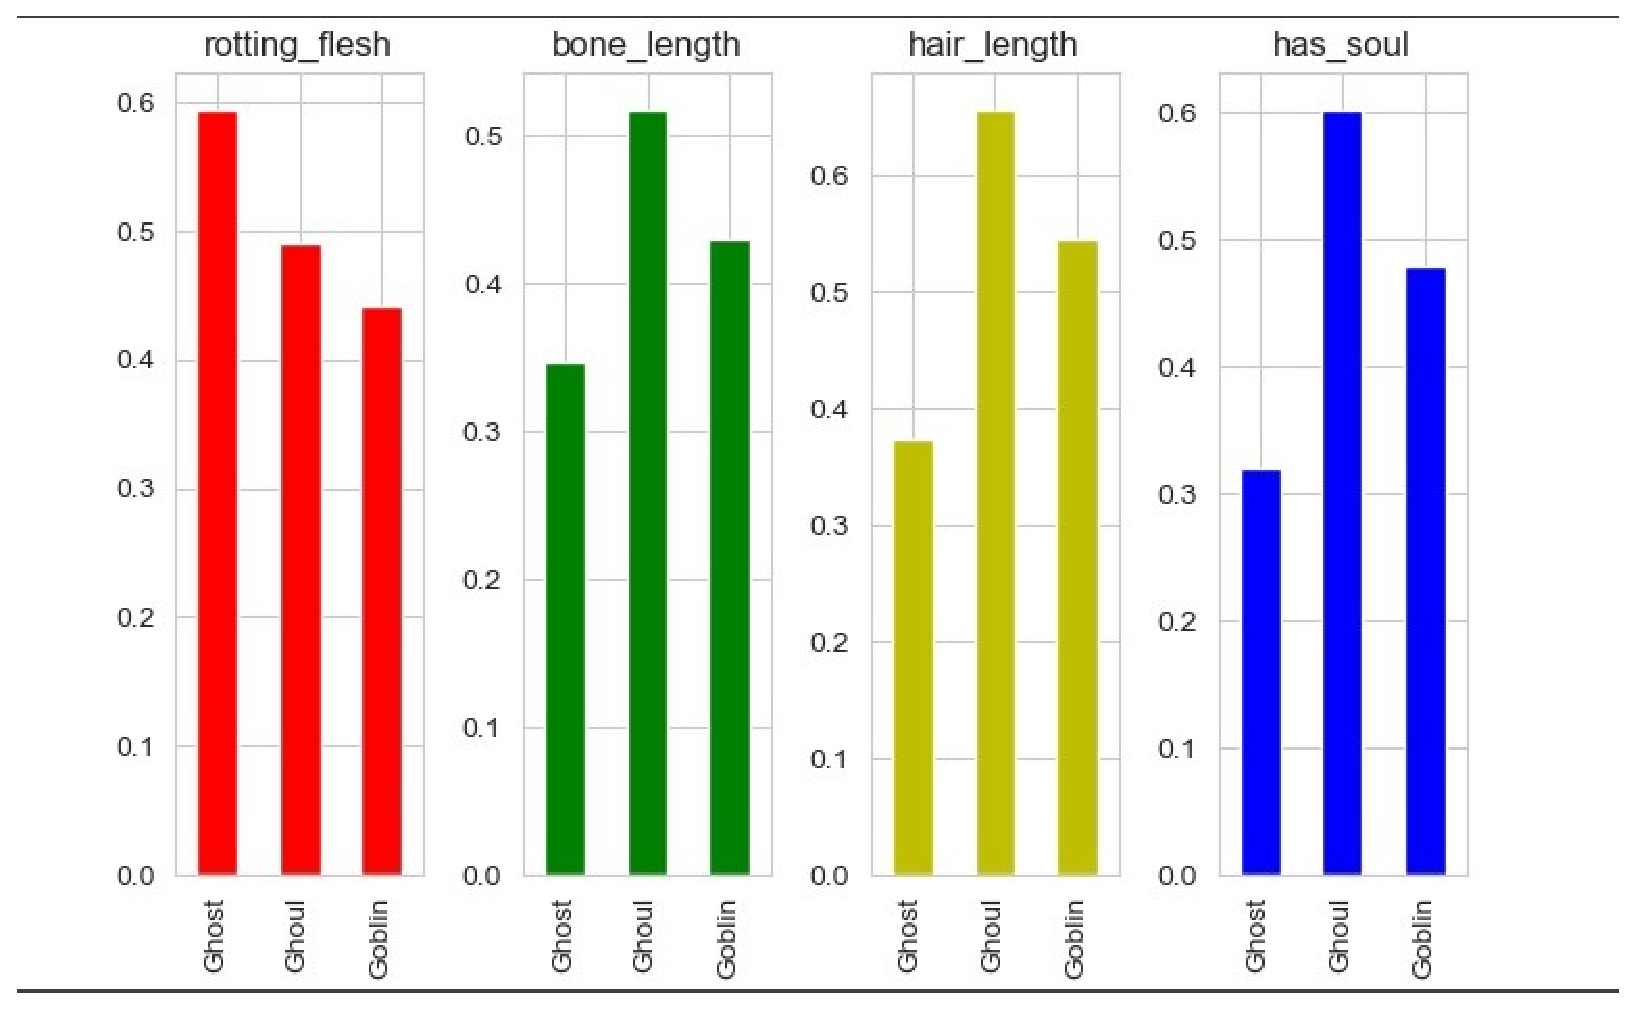
\includegraphics[scale=0.3]{figures/his_1.eps}
	\caption{Distribution of individual variables}\label{fig:his_1}
\end{figure}


\subsubsection{Boxplot}
\
 
When analyzing the data, 
the boxplot can effectively 
help us identify the characteristics of the data:
visually identify outliers in the dataset or
determine the data dispersion and 
bias of the data set. 
Through the figure ~\Cref{fig:boxplot}, 
we know that the outliers are very small,
so can be ignored.


\begin{figure}[htbp]
	\centering
	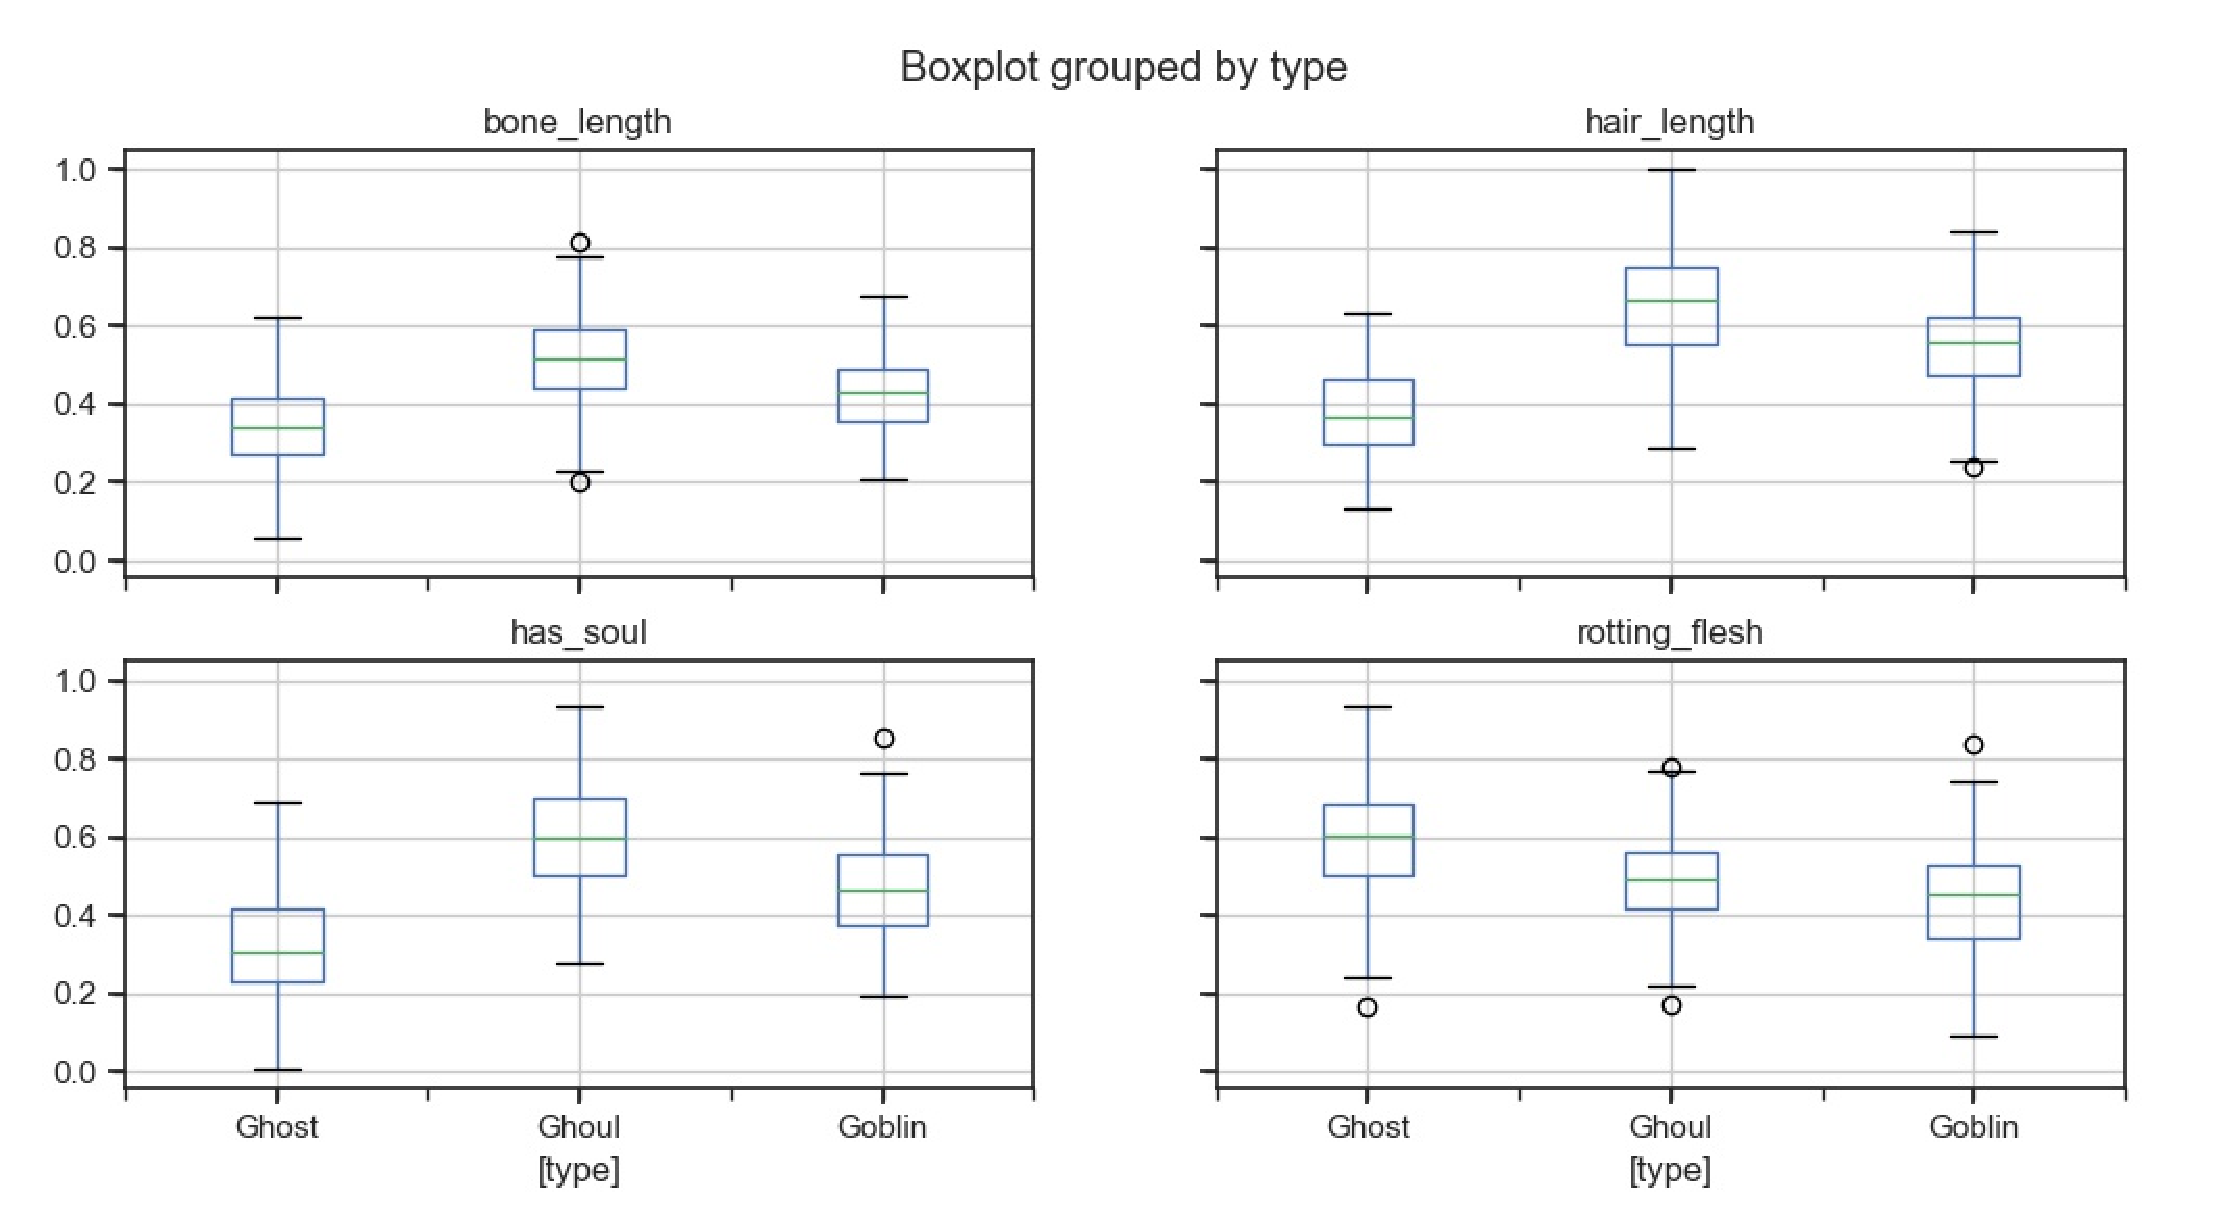
\includegraphics[scale=0.3]{figures/boxplot.eps}
	\caption{Boxplot of item_cnt_day and item_price}\label{fig:boxplot}
\end{figure}


\subsubsection{Scatterplot} 
\

This Scatterplot ~\Cref{fig:scatterplot} show 
that the daily sales volume 
of the product is mainly concentrated 
between 0 and 1, and the 
price of the product can also be concentrated. 
Use two sets of data to form multiple 
coordinate points, examine the distribution 
of coordinate points, and determine 
whether there is some correlation 
between the two variables or summarize 
the distribution pattern of the 
coordinate points. The scatter 
plot displays the sequence as a set of points.

\begin{figure}[htbp]
	\centering
	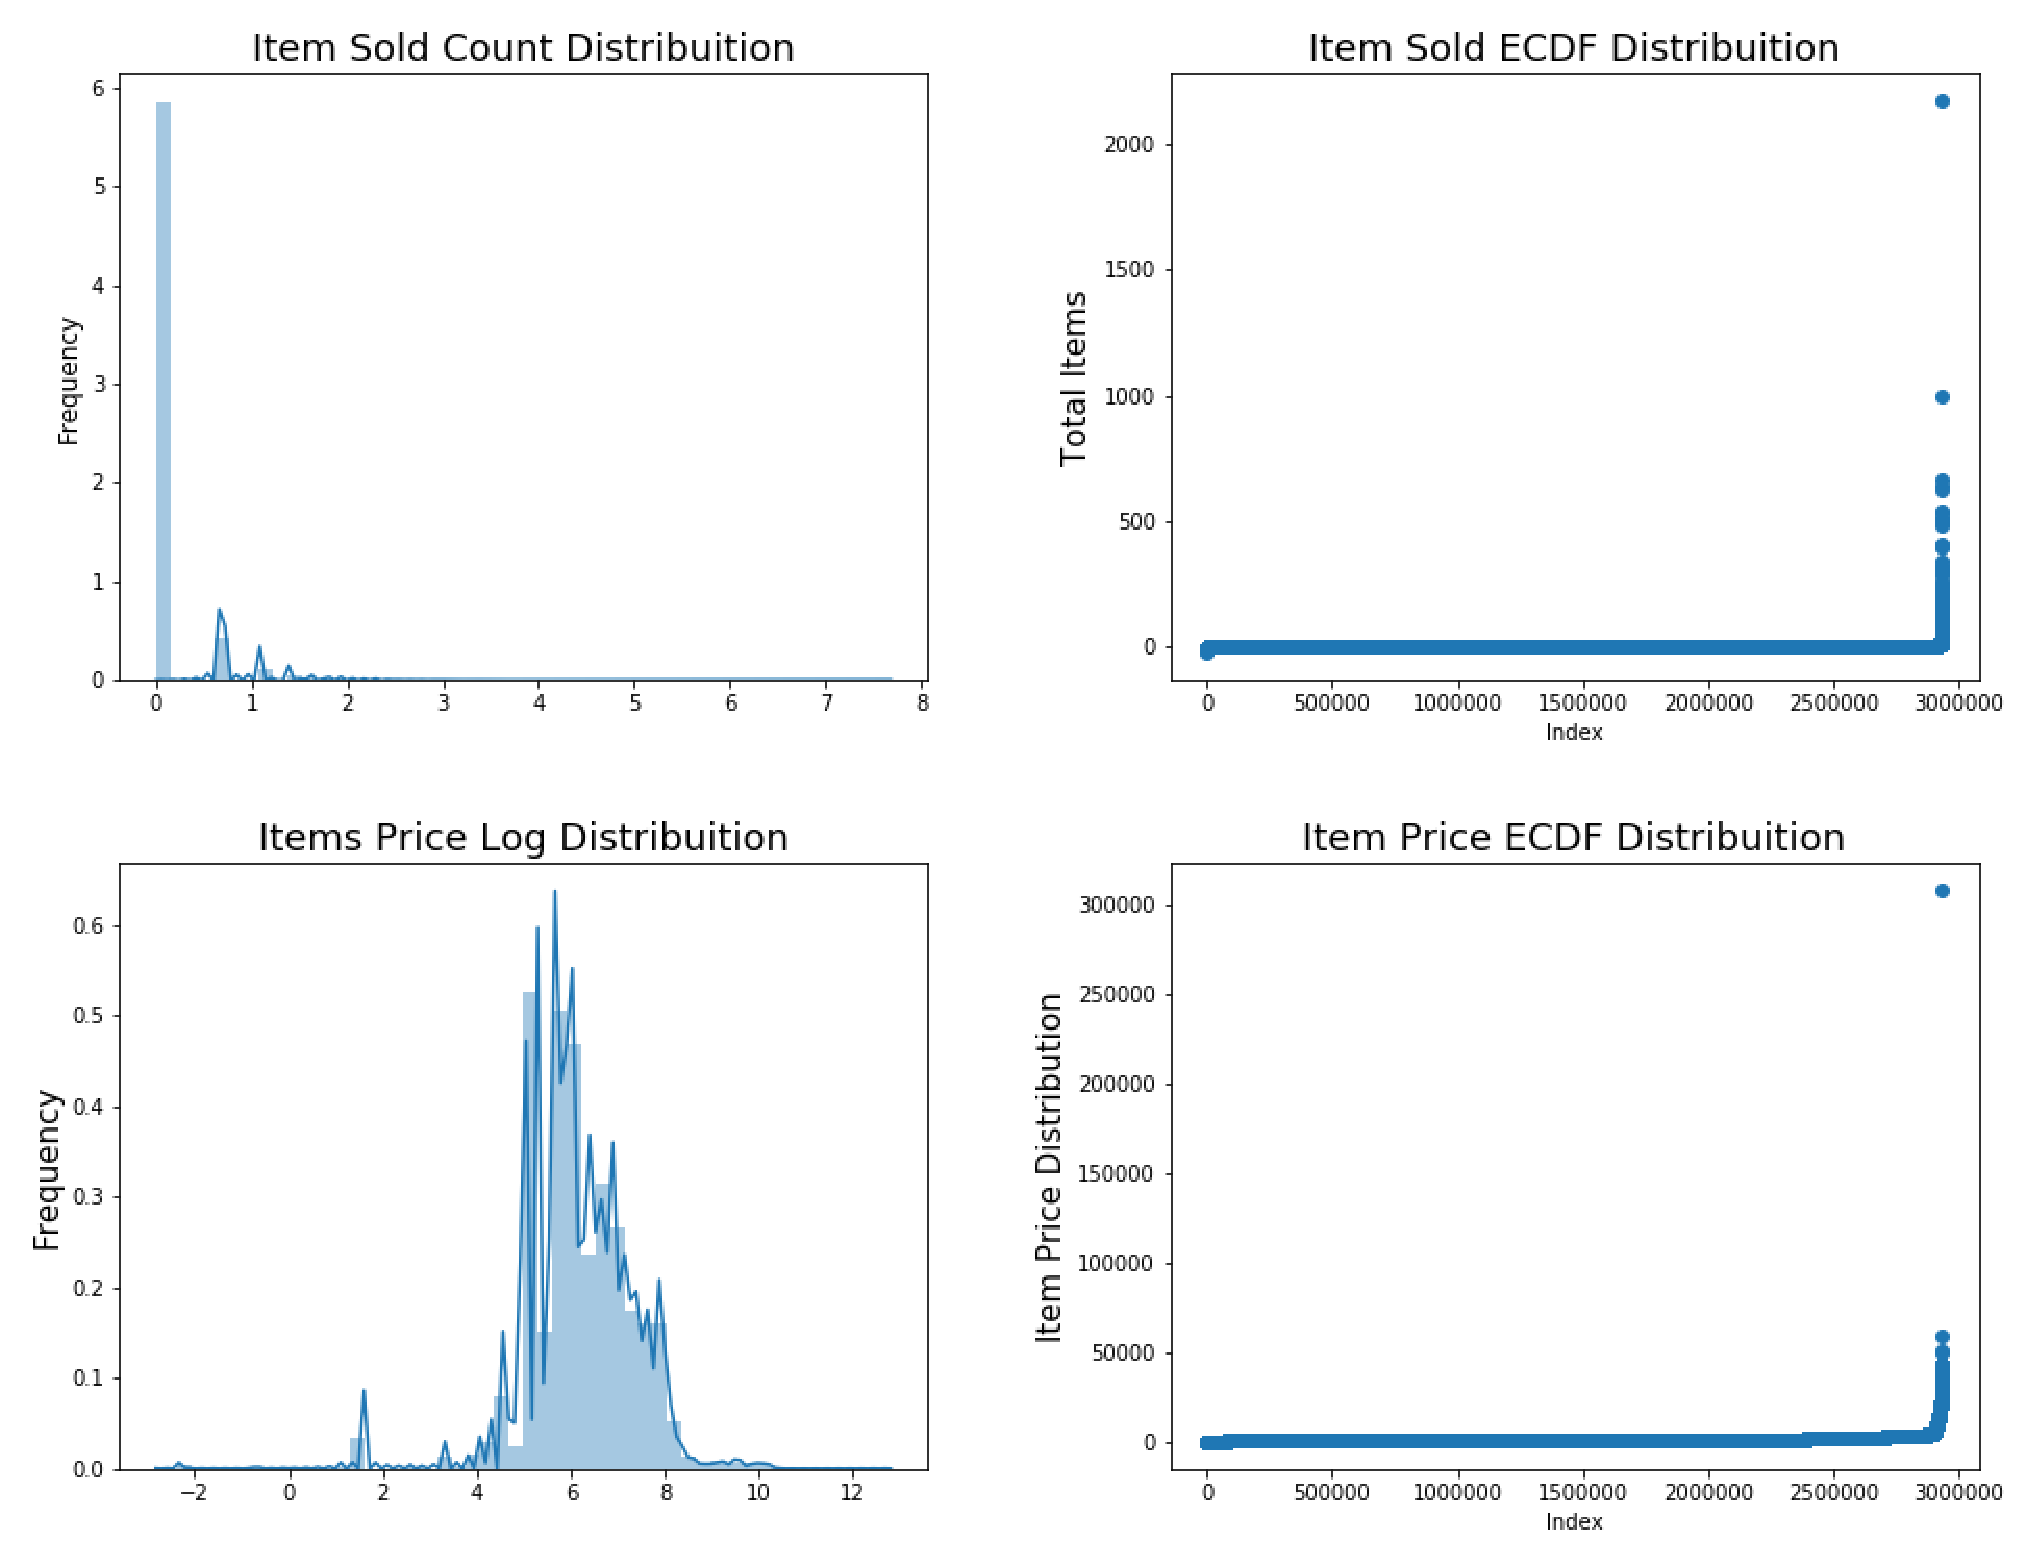
\includegraphics[scale=0.4]{figures/scatterplot.eps}
	\caption{Scatterplot of item_cnt_day and item_price}\label{fig:scatterplot}
\end{figure}

\subsubsection{Correllogram}
\

Correlogram is used to 
visually see the correlation metric 
between all possible pairs of numeric variables 
in a given dataframe. 
This figure ~\Cref{fig:corr} 
make it convenient for us to analyze features.
You can see that the item_cnt_day related 
to the target to be analyzed is item_id and item_price.

\begin{figure}[htbp]
	\centering
	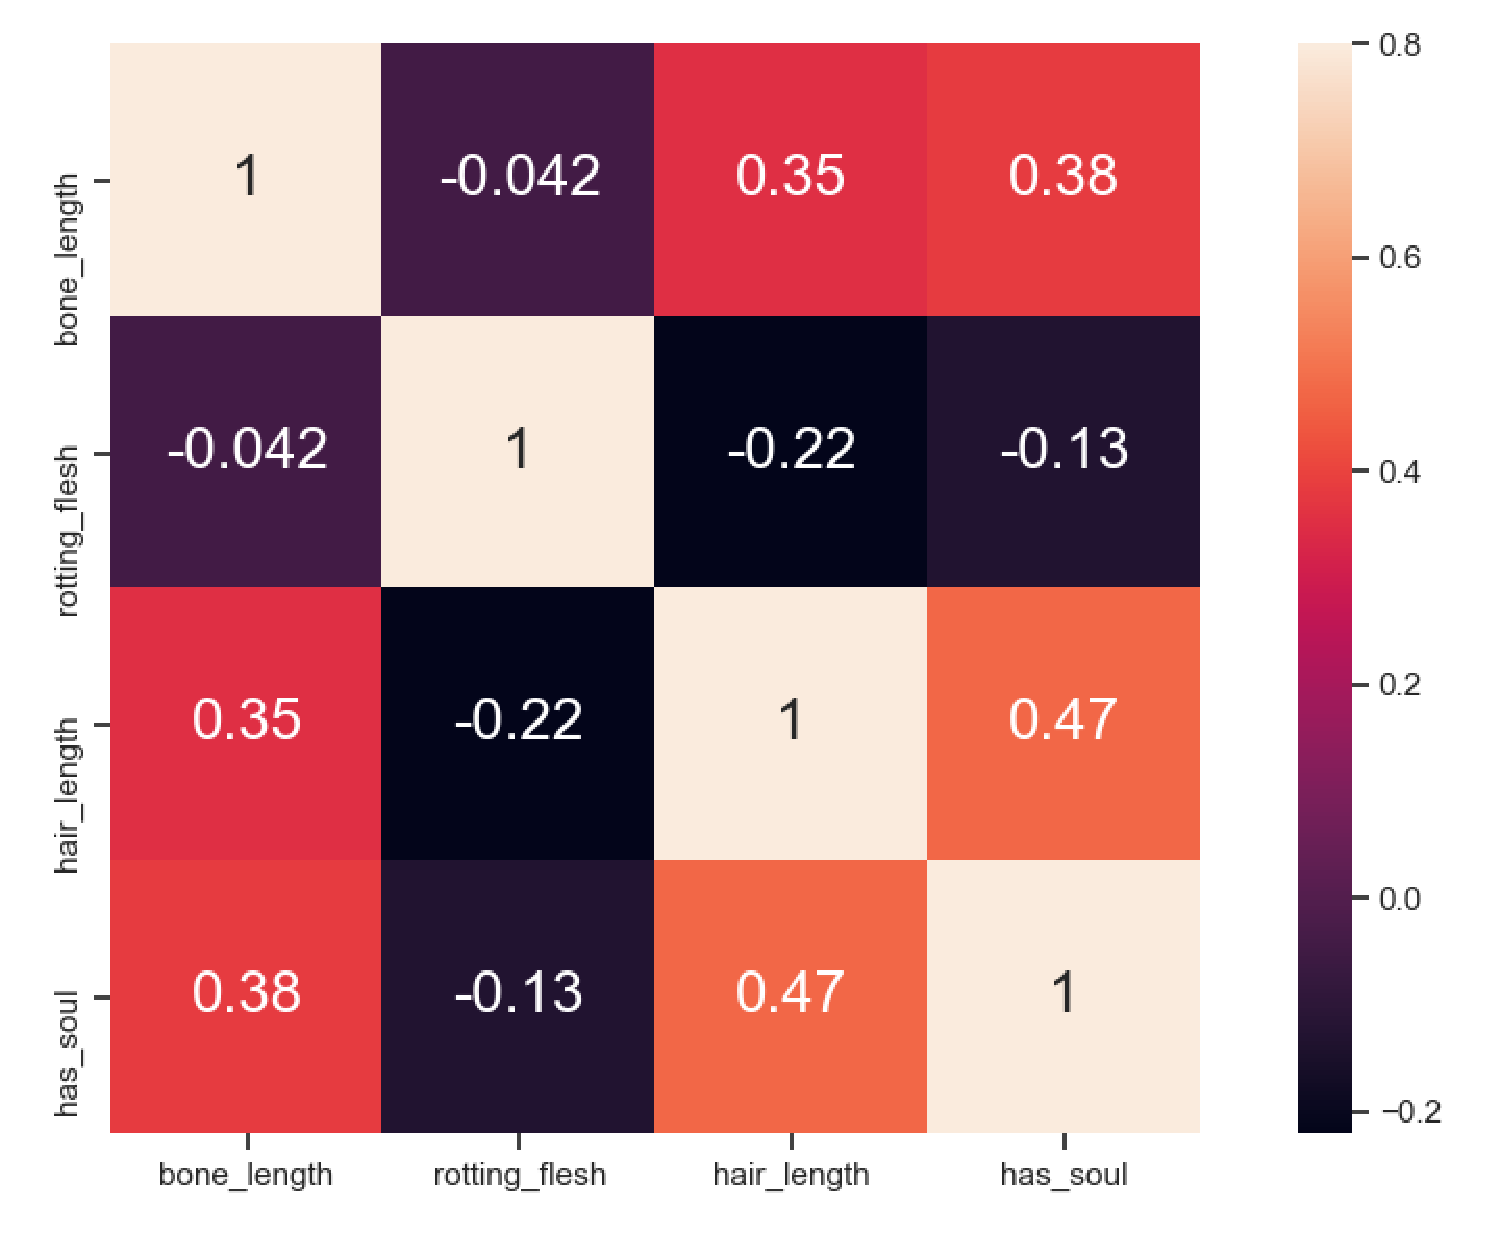
\includegraphics[scale=0.1]{figures/corr.eps}
	\caption{Correllogram}\label{fig:corr}
\end{figure}


\subsection{Data Preparation}



\subsubsection{Feature Selection}
\

Use the algorithm below to 
calculate the importance of features.
The following figure ~\Cref{fig:feature_importance}
is a histogram ordered by feature importance. 

\begin{algorithm}[htbp]
	\small
	\caption{Features Selection}
	\label{alg:features_selection}
	\begin{algorithmic}[1]
		\REQUIRE
		Features $X=\{ X_1, X_2, ... , X_n \}$,
		The number of tree node $M$,
		$GI_m$ Gini index of node $m$, 
		$ K $ the number of target,
		$ p_mk $ proportion of target $k$ in node $m$,
		$ VIM_{jm}^{\small(Gini)} $ the importance of feature $X_j$ in node $m$ ,
		$ n$ the tree number of RF.
		\ENSURE
		Variable Importance Measures $VIM_{j}^{\small(Gini)}$.
		\STATE
		Initialize $GI_m$ , 
		$VIM_{j}^{\small(Gini)} $;
		\FOR {$m \leftarrow 1...M$}
		\FOR {$k \leftarrow 1...K$}
		\STATE Compute the Gini index of node $m$
		$GI_m = \sum_{k=1}^{|K|} \sum_{k'\neq k} {p_{mk}}{p_{mk'}}=1- \sum_{k=1}^{|K|} p^2_{mk}$
		\ENDFOR
		\STATE Divide node m into node r and node l
		\STATE Compute the importance of feature $X_j$ in node $m$ 
		$VIM_{jm}^{\small(Gini)} = GI_m-GI_l-GI_r $
		\ENDFOR
		\FOR {$i \leftarrow 1...N$}
		\STATE Compute variable importance measures 
		$VIM_{j}^{\small(Gini)} = VIM_{j}^{\small(Gini)} + VIM_{ij}^{\small(Gini)}$
		\ENDFOR
		\RETURN $VIM_{j}^{\small(Gini)}$
	\end{algorithmic}
    %\caption{Feature Selection Algorithm}
\end{algorithm}

\begin{figure}[htbp]
	\centering
	%\graphicspath{{figures/}{mine/}}
	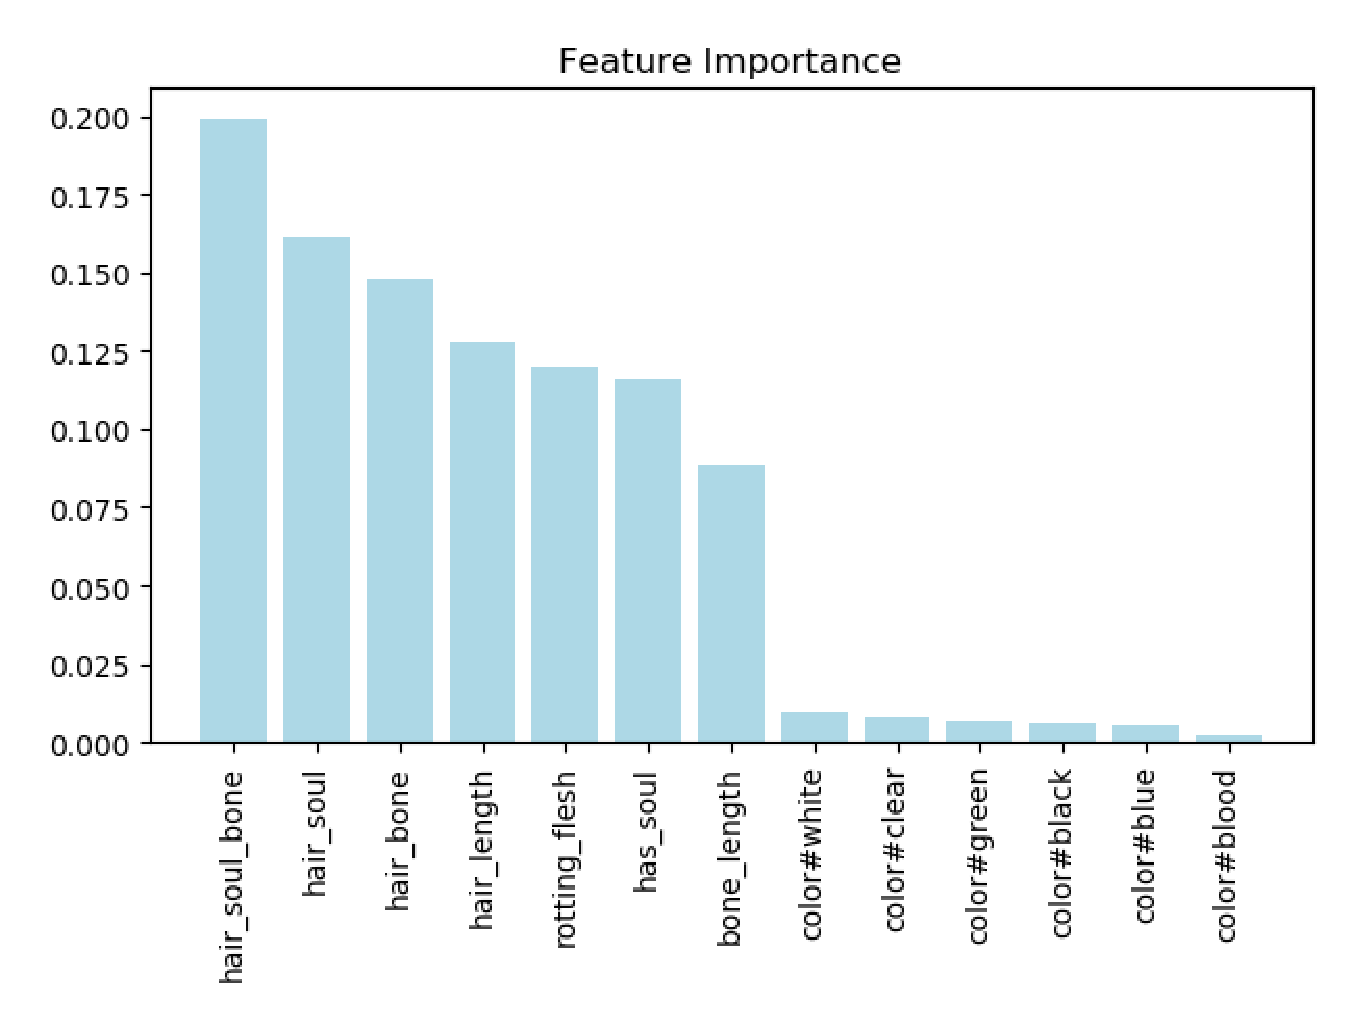
\includegraphics[scale=0.3]{figures/FEATURE.eps}
	\caption{Feature Importance}\label{fig:feature_importance}
\end{figure}

I take these features 
to form a new train datad.


\section{Methods}

There are many machine learning algorithms 
for Time-series problem. 
Choose the following algorithms
as the base models of ensemble model,show the most important parameters.

\begin{itemize}
    \item Base Models
	\
\begin{itemize}
	\item RandomForest 
	\item XGBoost
	\item LSTM
	\item Linear regression
	\item KNN
\end{itemize}
\item Ensemble Model
\end{itemize}
\subsection{Base Models}
\

The base models have many parameters,
select the some parameters that 
have a larger impact on 
the forecast results,
the use Grid Search to find 
the optimal paratemers set.	
The following is training result. 
\subsubsection{RandomForest}
\

Random forest is a classifier with 
multiple decision trees, and
the output is determined by 
the mode of the individual tree output.


\begin{description}
	\item[n_estimators] the number of decision trees
	\item[criteriom] criterion of choosing 
	the most appropriate node
	\item[max_depth] The maximum depth of the tree, 
	the default is None 
	\item[max_features] The feature that is divided 
	when selecting the optimal attribute 
	cannot exceed this value.
\end{description}
                  
	
\subsubsection{XGBoost}
\
 
XGBoost is to establish K regression trees 
so that the predicted value of 
the tree group is as close as possible to 
the true value (accuracy) and 
has the greatest generalization ability. 
From a mathematical point of view, 
this is a functional optimization, multi-target.

\begin{description}
	\item[learning_rate]  control the speed of each update
	\item[n_estimators] number of iterations
	\item[max_depth] the depth of tree
	\item[gamma] penalty factor%惩罚系数
	\item[subsample] the proportion of data used in 
		all training sets when training each tree
	\item[colsample_bytree] the proportion of features used 
		in all trees when training each tree
	\end{description}

\subsubsection{LSTM}
\

Long short-term memory (LSTM) is an artificial 
recurrent neural network (RNN) 
architecture used in the field of 
deep learning. LSTM has feedback connections. 
It can not only process single data 
points (such as images), but also entire 
sequences of data (such as speech or video). 
	
	
\begin{description}
	\item[units] Output dimension 
		the number of neurons in the i-th hidden layer
	\item[activation] activation function
	\item[recurrent_activation] Activation function applied to the loop step
	\item[use_bias] Boolean, whether to use bias term
\end{description}

\subsubsection{Linear regression}
\

Linear regression is a linear approach to 
modeling the relationship between a scalar 
response (or dependent variable) and one 
or more explanatory variables (or 
independent variables). 


\begin{description}
	\item[fit_intercept] whether to calculate the intercept for this model. If 
	set to False, no intercept will be used in calculations 
	the number of neurons in the i-th hidden layer
	\item[normalize] This parameter is ignored when fit_intercept is set to 
	False
	\item[copy_X] If True, X will be copied; else, it may be overwritten
	\item[n_jobs] The number of jobs to use for the computation
\end{description}

\subsubsection{KNN}
\

k-NN is a type of instance-based learning, 
or lazy learning, where the function is 
only approximated locally and all 
computation is deferred until classification. 


\begin{description}
	\item[n_neighbors] Number of neighbors to use by default for kneighbors 
	queries
	\item[weights] weight function used in prediction. Possible values
	\item[algorithm] Algorithm used to compute the nearest neighbors
	\item[leaf_size] Leaf size passed to BallTree or KDTree
\end{description}

\subsection{Ensemble Model}
\

To combine the base models as 1st level 
model predictions, I'll use a simple 
linear regression. As I'm only feeding 
the model with predictions 
I don't need a complex model.

\section{Experiment and Analysis}

In the Data Exploration, 
I has created some new feaures 
and found some outliers.
Because the number of outliers is very small, 
after ignoring the outliers, the features 
are selected for experiments based on their importance.
And use the trained models as 
the base models of ensemble model,
then do experiment.
%\WBJianginMarker

\subsection{Base Models Training Result}

The following are the best parameters and 
the best Score in training of 
the base models. 

\begin{itemize}
	\item Best Parameters of Models
	\begin{description}
		\item[RandomForest] 'n_jobs': '-1', 'max_depth': 15, 
		'random_state': 42, 'n_estimators': 25
		\item[XGBoost] 'max_depth':10, 
		'subsample':1,
		'min_child_weight':0.5,
		'eta':0.3, 
		'num_round':1000, 
		'seed':1,
		'silent':0,
		'eval_metric':'rmse'
		\item[LSTM] "batch_size":128,
		"verbose":2,
		"epochs":10
		\item[Linear regression] No other parameters required
		\item[KNN] n_neighbors=9, leaf_size=13, n_jobs=-1
	\end{description}


\subsection{Forecast Result of Base Models}
\

From the  ~\Cref{tbl:best_score_base_models_old},
it shows that the rmse of 
each model, RandomForest and XGBoost 
perform better, and there is not much 
difference between the other models.

\begin{table}[h]  \centering
	\caption{Best Score of the Base Models}
	\label{tbl:best_score_base_models_old}
	\begin{tabular}{ccccccc}
		%\bottomrule
		\toprule
		& RandomForest & XGBoost & LSTM & Linear regression & KNN\\
		\midrule
		Train rmse & 0.8358 & 0.8327 & 0.9276 & 0.8572 & 0.6976\\
		Validation rmse & 0.8810 & 0.8959 & 0.6611 & 0.8806 & 0.8946\\
		\bottomrule
	\end{tabular}
\end{table}
\end{itemize}

\subsection{Forecast Result of Ensemble Model }
\

Ensemble model means using 
more than 1 model to finish the prediction.
The train rmse is 0.764973649571408.

\section{Conclusion}

\begin{itemize}
	\item Exploratory data analysis is 
	very important for the competition,
	Discover the imperfections of the 
	data and have a certain understanding 
	of the overall appearance of the data, 
	which will help later modeling and analysis. 
	\item The data that we have,
	needed processed in many cases.
	Data preprocessing includes 
	deal with missing data and outliers, 
	We must think carefully about the outliers, 
	such as ignoring them.
	\item The most important thing is
	feature engineering.
	We have to think carefully and 
	deal with outliers, such as ignoring 
	or deleting them.
	\item There is no best model, 
	only the best model. We should 
	try as many models as possible to 
	get the best prediction results. 
	\item Feature engineering is very 
	important and even plays a decisive 
	role in this competition.
	\item The Ensemble model may perform better 
	than a single model when dealing 
	with some complex problems.	
\end{itemize}

%\lstset{language=python}         
%\begin{lstlisting}[frame=single]  % Start your code-block
%rf = RandomForestClassifier(random_state = 0)
%clf = GridSearchCV(rf, param_grid = params, scoring = accuracy_scorer, cv = 10, n_jobs = -1)
%clf.fit(X_train, y_train)
%y_pred = clf.predict(X_test)
%\end{lstlisting}










